\section{Applications}

\subsection{Overview}

Traditional applications can not achieve complicated and efficient goals due 
to the limited processing power and memory space of sensors.

In {\sdn}, applications for wireless sensor networks are inspired by 
greater potential with the UAV based SDN controller. The central controller
helps sensors execute complex calculations such as AI model training, as well 
as store global information. Besides, UAVs have flexible features and can deploy 
tasks to sensors by one-hop communication directly. Thus it enables the sensor network
to achieve much more intelligent applications.

In {\sdn}, applications can be found for a variety of purposes, including routing, AI node selection,
Ai energy prediction, multi-tasks and network diagnosis. We design all these applications and provide 
easy-to-use interfaces to users as in Table \ref{API}.



\subsection{Routing}

\begin{table}[htbp]
	\caption{Flow Table}
	\label{FT}
	\centering
	\scalebox{0.9}{
	\begin{tabular}{|l|l|l|}
		\hline
		Header Fields & Counters & Actions \\
		\hline
		\end{tabular}
	}
\end{table}

\begin{table}[htbp]
	\caption{Header Fields}
	\label{HF}
	\centering
	\scalebox{0.9}{
	\begin{tabular}{|l|l|l|l|l|}
		\hline
		Ingress port & Ether Source & Ether Dst &IP src & IP dst \\
		\hline
		\end{tabular}
	}
\end{table}

Actions:
\begin{itemize}
\item	Forward
\item	Drop
\item	Report
\end{itemize}

\subsection{AI Node Selection}

\subsubsection{Motivation}

\subsubsection{Design}

Greedy selection algorithm.

\begin{algorithm}
\caption{Greedy Selection Algorithm}
\label{Greedy}
\begin{algorithmic}[1]
\STATE Input: Sensor set $N$, Selected set $M$, Target area $\Omega$, Covering area $\Phi$;
\STATE Initialize : $M = \emptyset$, $\Phi = \emptyset$
\WHILE {$M \neq N$}
    \IF{$\Phi = \Omega $}
        \STATE break; $\backslash$$\backslash$ selected set has been found
    \ENDIF
    \IF{$\forall n_i \in (N-M) : range(n_i) \subset \Phi$}
    	 \STATE break;$\backslash$$\backslash$ Cannot cover the target area;
    \ENDIF
    \STATE Find $n_i : argmax(\Phi \cap range(n))$, $n_i \in (N-M)$;
    \STATE $\Phi = \Phi \cup {n_i}$
\ENDWHILE
\STATE Output: $M$;
\end{algorithmic}
\end{algorithm}

SRSSS AI algorithm selection.

\begin{figure}[htbp]
	\centering
	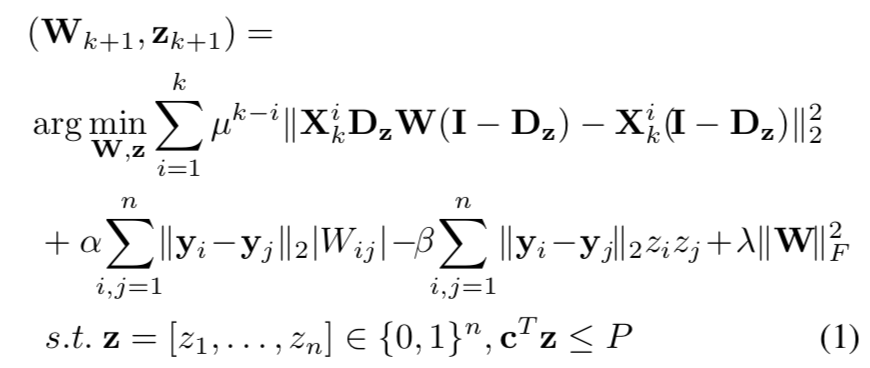
\includegraphics[width=2in]{Figure/OF}
	\caption{Objective function.}
	\label{system}
\end{figure}


**************

AI helps creating smarter sensor systems.

AI systems have been improving, and new advances in machine intelligence are creating seamless interactions between people and digital sensor systems.

 In sensor systems, applications can be found for a variety of tasks, including selection of sensor inputs, interpreting signals, condition monitoring, fault diagnosis, machine and process control, machine design, process planning, production scheduling, and system configuring. Some examples of specific tasks undertaken by expert systems are:
* Assembly 
* Automatic programming 
* Controlling intelligent complex vehicles  
* Planning inspection 
* Predicting risk of disease 
* Selecting tools and machining strategies 
* Sequence planning 
* Controlling plant growth. 

AI can increase effective communication, reduce mistakes, minimize errors, and extend sensor life.



The tools and methods described have minimal computation complexity and can be implemented on small assembly lines, single robots, or systems with low-capability microcontrollers. These novel approaches proposed use ambient intelligence and the mixing of different AI tools in an effort to use the best of each technology. The concepts are generically applicable across many processes.


minimum energy, data loss, reliability, robustness, etc., in place during the design and operation of wireless sensor networks

a specific set of protocols for medium access, localization and positioning, time synchronization, topology control, security and routing are identified based on the current configuration of the network, the requirements of the application and the topology of their deployment.

\subsection{AI Energy Prediction}

\subsubsection{Motivation}

\subsubsection{Design}

\subsection{Multi-tasks}

\subsubsection{Motivation}

Wireless sensor networks (WSN)  generally comprise of a group of 
spatially dispersed sensors. In a wireless sensor network, 
sensor nodes are equipped with various 
types of sensors monitoring and recording 
environmental conditions like temperature, sound, sunlight,
humidity, etc.

A given sensing task involves multiple sensors to 
achieve a certain quality-of-sensing.
Generally, an efficient task scheduling for the nodes is that nodes 
are able to perform multiple tasks simultaneously. 
For example, sensors deployed in a grove are assigned tasks to collect
sunlight, temperature and humidity data and these tasks require different 
number of  nodes with respective sensing range, rate and duration.
However, traditional sensor networks are not suitable to conduct this 
multi-tasks due to the limitations of computation complexity for task 
arrangement of each node.

In our {\sdn} system, we implement the multi-tasks application 
with the help of the central controller. The SDN controller
maintains programmable task scheduling and management
modules while sensor nodes are loaded with interfaces to
receive task control instructions.     

\subsubsection{Design}

A deployed wireless sensor networks are usually assigned  


A sensor node may have different sensing ranges for different tasks.


There are several practical requirements.

Different tasks have different requirements, including time, sensing range, sensing ratio, etc.

For example tasks like sunlight collection only need to be carried out during the daytime.

Our system provide a task scheduling to 

Sensors are usually assigned multi-tasks.

Sensors are assigned tasks to monitor a specific area.

Different tasks have different requirements, including time, density, etc.

\begin{itemize}
\item[nodeset] kk
\item[sensing rate] energy
\item[sensing range] processing
\item[sensing duration] memory
\end{itemize}

Task scheduler do the arrangement. 

Task buffer.

Task queue.

Scheduling table.

...

\subsection{Network Diagnosis}

Diagnose the network.
